\documentclass{article}
\usepackage[T1]{fontenc}
\usepackage[utf8]{inputenc}
\usepackage[french]{babel}
\usepackage{amsthm}
\usepackage{amsmath}
\usepackage{hyperref}
\usepackage{graphicx}
\usepackage{subcaption}
\graphicspath{ {.} }

\title{Coursera - Machine Learning}
\author{Benjamin Kermani}

\theoremstyle{definition}
\newtheorem{definition}{Definition}[section]

\begin{document}
\maketitle
\begin{center}
Notions abordées dans ce cours:
\end{center}
\begin{itemize}
\item[$\bullet$] Apprentissage supervisé
	\begin{itemize}
		\item Régression linéaire
		\item Régression logistique
		\item Réseaux de neurones
		\item Machine à vecteurs de support (SVM)
	\end{itemize}
\item[$\bullet$] Apprentissage non-supervisé
	\begin{itemize}
		\item K-Means
		\item Analyse en composantes principales (PCA)
		\item Détection d'anomalies
	\end{itemize}
\item[$\bullet$] Domaines d'application
	\begin{itemize}
		\item Systèmes de recommandations
		\item Machine learning à grande échelle (grand volume de données)
	\end{itemize}
\item[$\bullet$] Conseils de conception
	\begin{itemize}
		\item Biais/variance
		\item Régularisation
		\item Décisions d'amélioration et de priorisation
		\item Evaluer un algorithme d'apprentissage
		\item Courbes d'apprentissage
		\item Analyse des écarts
		\item Analyse d'une pipeline d'un algorithme de machine learning
	\end{itemize}
\end{itemize}
\newpage
\tableofcontents
\newpage
\section{Introduction}
\begin{definition}{Machine Learning}
"Science of getting computers to learn, without being explicitly programmed".
\end{definition}
"A computer program is said to learn from experience E with respect to some class of tasks T and performance measure P, if its performance at tasks in T, as measured by P, improves with experience E."	\par
\subsection{Différence avec le Deep Learning}
Le Deep Learning est un sous-ensemble du Machine Learning, la principale différence réside dans le fait qu'un programme de Deep Learning est capable de déterminer, grâce à un réseau de neurones, si une prédiction est précise ou non, sans l'assistance d'un ingénieur.\par
\subsection{Apprentissage Supervisé}
On entend par apprentissage supervisé, que le jeu de données donné à l'algorithme contient les "bonnes réponses". On sait à quoi ressemble une "bonne" sortie, avec l'idée qu'il y a une relation entre notre entrée et la sortie.\par \bigskip
Le problème de la prédiction du prix d'une maison en fonction de sa taille est ce que l'on appelle un problème de régression
\begin{definition}{Problème de régression}
"Predict continuous valued output."
\end{definition}
 	Tandis que le problème du "cancer du sein" est un problème de classification
 	\begin{definition}{Problème de classification}
"Predict discrete valued output."
\end{definition}

\begin{figure}[h!]
  \centering
  \begin{subfigure}[b]{0.49\linewidth}
    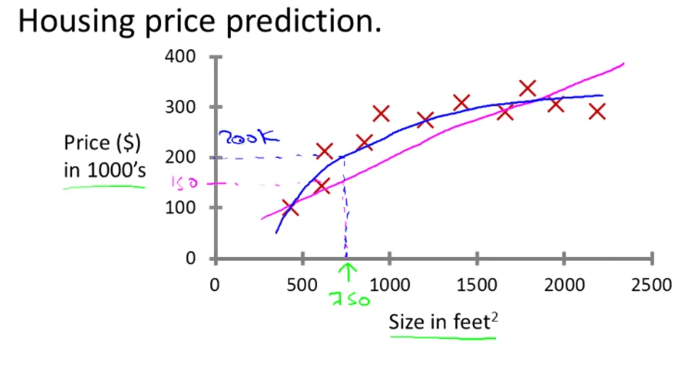
\includegraphics[width=\linewidth]{supervised}
    \caption{Problème de régression}
  \end{subfigure}
  \begin{subfigure}[b]{0.49\linewidth}
    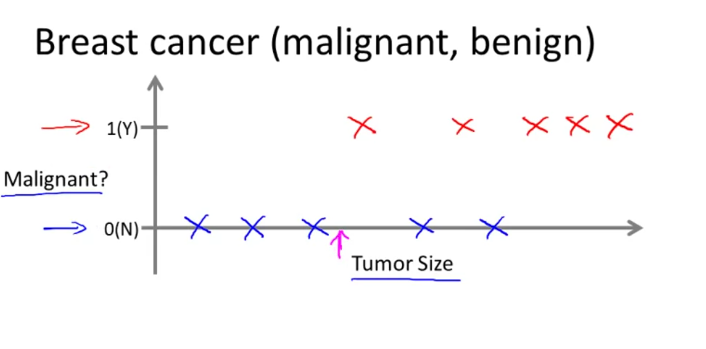
\includegraphics[width=\linewidth]{supervised2}
    \caption{Problème de classification}
  \end{subfigure}
\label{fig:coffee}
\end{figure}
\subsection{Apprentissage Non-Supervisé}
\begin{definition}{Apprentissage non-supervisé
Lorsqu'on donne une grande quantité de données, non-étiquetées, à un algorithme et qu'on lui demande de découvrir les structures sous-jacentes à ces données.}
\end{definition}
Cette méthode de résolution permet de résoudre des problèmes dont on a peu ou pas d'informations sur la forme de sa solution. \par
\newpage
\section{Régression Linéaire à Une Variable}
\subsection{Modèle et Fonction de Coût}
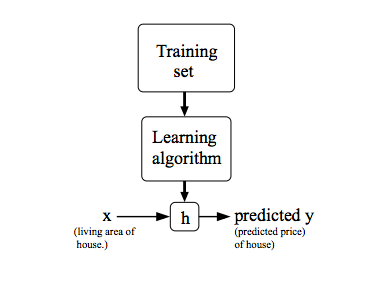
\includegraphics{model} \par
On utilisera $x^{(i)}$ pour dénoter les entrées, $y^{(i)}$ pour les sorties, et $(x^{(i)},y^{(i)})$ pour la ième expérience. \par
\paragraph{Fonction de coût}
Elle permet de trouver la meilleure fonction affine pour représenter nos données \par
On va chercher à minimiser la fonction de coût $J(\theta_0 , \theta_1)$. Cette fonction prend la moyenne de la différence entre la fonction d'évaluation, "d'hypothèse" $h_\theta (x_i)$ et les sorties $y_i$ : \par
\begin{equation} \label{eu_eqn}
J(\theta_0 , \theta_1) = {1\over 2n} \sum_{i=1}^{n} (h_\theta (x_i) - y_i)^2
\end{equation}
Cette fonction est également appelée: "squared error function"
\paragraph{Fonction de coût : Intuitions}
Soit une équation du type $h(x) = \theta_1x + \theta_0$ Lorsqu'on pose $\theta_0 = 0$, on remarque que notre fonction de cout $J(\theta_1)$ est une équation à 2 dimensions. \par
Ainsi lorsque $\theta_0 \ne 0$, On obtient une figure en 3D ("contour plot"). \par
\subsection{"Parameter Learning"}
\subsubsection{Descente de Gradient}
La descente de gradient est un algorithme qui permet de minimiser la fonction de coût $J(\theta_0,\theta_1)$\par
Il garantit de trouver \textbf{un optimum local, i.e un minimum local.} On effectue des pas et on cherche le point sur la surface (le "contour plot" de la fonction de coût), qui minimise le plus sa valeur, on itère jusqu'à atteindre un minimum local\par
\begin{equation} \label{eu_eqn}
\theta_j:=\theta_j - \alpha\frac{\partial }{\partial \theta_j}J(\theta_0,\theta_1)
\end{equation}
Où $j= 0,1$ représente les index des variables et $\alpha$ le "taux d'apprentissage", il contrôle la "grandeur" des pas que l'on fait à chaque itération. \par 
Il faut mettre à jour les valeurs des paramètres \textbf{simultanément}, sans quoi la valeur de la fonction de coût changerais pour les autres paramètres \par
\paragraph{Descente de gradient : Intuitions}
Si l'on cherche un minimum local, alors la fonction $J(\theta_0,\theta_1)$ décroît et par conséquent, la valeur de $\frac{\partial }{\partial \theta_j}J(\theta_0,\theta_1)$  est négative, d'où le signe moins dans l'algorithme.\par
Si $\alpha$ est trop grand, il peut faire échouer la convergence et même faire diverger la fonction de coût. si $\alpha$ est trop petit, la convergence sera très lente.\par 
Si $\alpha$ est fixé, l'algorithme converge quand même vers un minimum local puisque plus on se rapproche d'un minimum, plus la dérivée partielle, $\frac{\partial }{\partial \theta_j}J(\theta_0,\theta_1)$ décroît (la pente est moins raide).\par
\subsubsection{Descente de Gradient Dans le Cas d'une Régression Linéaire}
On va utiliser l'algorithme de "descente de gradient" pour notre fonction de coût préalablement établie. En trouvant les dérivées partielles de notre fonction de coût $J(\theta_0,\theta_1)$, on trouve :
\begin{equation} \label{eu_eqn}
\theta_0:=\theta_0 - \alpha\frac{1}{n}\sum_{i=1}^{n} (h_\theta (x_i) - y_i)
\end{equation}
\begin{equation} \label{eu_eqn}
\theta_1:=\theta_1 - \alpha\frac{1}{n}\sum_{i=1}^{n} (h_\theta (x_i) - y_i)*x_i
\end{equation}
Cette version est appelée "Batch Gradient Descent", puisqu'on utilise tous nos tuples de données.\par
Note : Dans notre cas, la fonction de coût ne comporte qu'un minimum global (et aucun local).\par
\newpage
\section{Rappels : Algèbre Linéaire}
Dimensions d'une matrice = nombre de lignes * nombre de colonnes
\paragraph{Addition de matrices}
Pour additionner deux matrices, leurs dimensions doivent être\textbf{ similaires}
\paragraph{Multiplication de matrices}
Soit une matrice A de dimensions (n,m) \par
Soit une matrice B de dimensions (m,p) \par
Pour pouvoir multiplier la matrice A par la matrice B, il faut que le nombre de colonnes de A soit égale au nombre de lignes de B.\par
La matrice résultat M aura pour dimensions (n,p). Soit autant de lignes que la matrice A et le même nombre de colonnes que la matrice B
\begin{equation}
A =
\begin{bmatrix} 
1 & 2 & 3 \\
4 & 5 & 6 \\
7 & 8 & 9
\end{bmatrix}
\begin{bmatrix} 
a\\
b \\
c
\end{bmatrix}
=
\begin{bmatrix} 
1*a + 2*b + 3*c\\
4*a + 5*b + 6*c\\
7*a + 8*b + 9*c
\end{bmatrix}
\end{equation}
\paragraph{Propriétés sur la multiplication de matrices}
\begin{itemize}
  \item Les matrices ne sont pas commutative : $A*B \ne B*A$ (sauf si B= $I_D$)
  \item Les matrices sont associative : $(A*B)*C = A*(B*C)$
\end{itemize}
\paragraph{Matrice Inverse}
La matrice inverse de A, dénotée $A^{-1}$, a pour propriété: 
\begin{equation}
A^{-1}A = AA^{-1} = I_D
\end{equation}
$\forall  M_{n*n}$, tel que $det(M) \neq 0$ alors la matrice M est inversible.
\paragraph{Transposée d'une matrice}
On appelle transposée d'une matrice de type $(n,p)$ et de terme général , $a_{i,j}$ la matrice notée ${^t}A$ de type $(p,n)$ , dont le coefficient de la i-ème ligne et de la j-ème colonne est $a_{j,i}$.\par Autrement dit, on permute le rôle des lignes et des colonnes.
\begin{equation}
{^t}
\begin{bmatrix} 
2 & -1 & 3 \\
0 & -4 & 5 
\end{bmatrix}
=
\begin{bmatrix} 
2 & 0\\
-1 & -4 \\
3 & 5
\end{bmatrix} 
\end{equation}
\newpage
\section{Régression linéaire à plusieurs variables}
\subsection{"Multivariate Linear Regression"}
Nous avons maintenant $n$ variables :
\begin{equation}
h_\theta(x) = \theta_0 + \theta_1 x_1 +...+\theta_n x_n
\end{equation}
Notre équation d'hypothèse devient:
\begin{equation}
h_\theta(x) = {^t}[\theta][x]
\end{equation}
Avec  $x_0=1$ par convention.
L'équation de descente de gradient quant à elle devient : 

\begin{equation}
\theta_j:=\theta_j - \alpha\frac{1}{n}\sum_{i=1}^{n} (h_\theta (x^{(i)}-y^{(i)})x_j^{(i)} forj:=0..n
\end{equation}
\subsection{Améliorer la convergence}
\paragraph{Mise à l'échelle des paramètres :}
Pour obtenir une convergence plus rapide il est important que chaque paramètre soit sur une même échelle de valeurs. En pratique, il faut que les valeurs de chaque paramètre se situent dans l'intervalle $-1 \leq x \leq 1$
Pour se faire on peut utiliser sur tous les paramètres (sauf $x_0$) la \textbf{moyenne normalisée} :
\begin{itemize}
	\item \textbf{Debugger :} Faire un graphe Nb.iterations vs $J(\theta)$, si $J(\theta)$ croît, alors il faut probablement diminuer le paramètre $\alpha$
	\item \textbf{Test de convergence automatique:} On considère que $J(\theta)$ a convergé si pour une itération, $J(\theta)$ décroît moins qu'une certaine valeur $\epsilon \leq 10^{-3}$
	\item \textbf{Régression polynomiale : } C'est l'idée de choisir ses paramètres pour obtenir un meilleur modèle. En fonction de la représentation des données (cf.nuage de points), certaines équations polynomiales s'adapteront mieux à notre modèle que d'autres.
\end{itemize}
\subsection{Équation normale}
C'est une autre méthode qui permet de minimiser la fonction de coût $J(\theta)$. On prend la dérivé de $J(\theta)$ pour chaque $\theta_j$ et on résout le système pour $\theta=0$ .La formule est la suivante :
\begin{equation}
\theta = (X^{T}X)^{-1}X^{T}y
\end{equation}
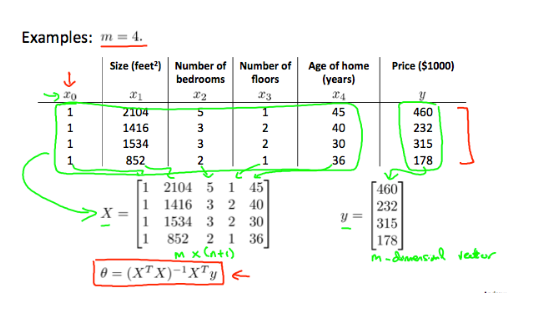
\includegraphics{normal-equation}
Cette méthode n'a pas besoin de \textbf{mettre à l'échelle ses paramètres}
\paragraph{Avantages et quand l'utiliser :}
\begin{center}
\begin{tabular}{|l|c|r|}
  \hline
  Descente de gradient  & Équation normale \\
  \hline
  Besoin de choisir alpha & Pas besoin de choisir alpha \\
  Besoin de beaucoup d'itérations & Instantané \\
  $O(kn^2)$ & $O(n^3)$ pour faire l'inverse de $X^{T}X$ \\
  A utiliser quand n est grand & Lent quand n est grand \\
  \hline
\end{tabular}
\end{center}
\newpage
\section{Rappels : Matlab/Octave}
\subsection{Opérations de base}
\begin{itemize}
	\item \textbf{Instanciée une variable sans l'afficher : } Rajouter ";"
	\item \textbf{afficher une variable : } disp(X)
	\item \textbf{afficher un flottant avec une certaine précision : } disp(sprintf('\%0.2f',X)
	\item \textbf{Vecteurs et Matrices : }
	\begin{itemize}
		\item \textbf{Créer une matrice/ un vecteur :} A = [1 2 ; 3 4]
		\item \textbf{Créer un vecteur entre 2 valeurs :} A = 1:6
		\item \textbf{Créer un vecteur incrémentalement  :} A = 1:0.1:2
		\item \textbf{Opérations sur les matrices :}
			\begin{itemize}
				\item ones(2,3) : Génère une matrice M(2x3) de 1
				\item rand(1,3) : Génère une matrice M(1,3) avec des valeurs aléatoires entre 0 et 1
				\item magic(N) : Génère une matrice de dimensions N dont les colonnes, lignes et la diagonale ont les même valeurs
				\item eye(N) : Génère la matrice identité de dimensions N
				\item size(X) : Retourne les dimensions de la matrice X
				\item \textbf{accéder à un élément :} X(3,2) : accède à l'élément de la 3ème ligne et de la 2nd colonne
				\item \textbf{accéder à tous les éléments d'une ligne/colonne :} X(2,:) : Accède à tous les éléments de la 2nd ligne
				\item \textbf{accéder à tous les éléments de plusieurs lignes/colonnes :} X([1 3], :) : Retourne tous les éléments de la 1ère et 3ème lignes
				\item \textbf{Changer la matrice en un vecteur colonne : } X(:)
			\end{itemize}
		
	\end{itemize}
	\item \textbf{Opérations sur les vecteurs :}
		\begin{itemize}
			\item length(v) : dimensions du vecteur
		\end{itemize}
	\item \textbf{Afficher un histogramme: } hist(X)
	\item \textbf{Charger un fichier : } load nomFichier
	\item \textbf{Afficher les variables utilisées : } who [whos pour plus d'informations]
	\item \textbf{Supprimer une varaible : } clear nomVariable [clear supprime toutes les variables]
	\item \textbf{Sauvegarder une variable dans un fichier : } save nomFichier nomVariable [ save nomFichier.txt nomVariable -ascii ]	
\end{itemize}
\subsection{Calculs sur les données}
"." : Element-wise \par
"'" : Transposed 
\begin{itemize}
	\item \textbf{Multiplier 2 matrices : } C = A*B
	\item \textbf{Multiplier chaque élément :} C = A .*B : Prend chaque élément de A et le multiplie par l'élément à l'index correspond de la matrice B  
	\item \textbf{Maximum et index d'un vecteur :} [val, ind] = max(X)
	\item \textbf{Index d'éléments vérifiant une condition (vecteur) : } find (X<3)
	\item \textbf{Index d'éléments vérifiant une condition (matrice) : } [r, c] = find (X>=7)
	\item \textbf{Opérateurs : } sum(X), prod(X), floor(X), ceil(X)
	\item \textbf{Maximum "column-wise" (matrice) :} max(X,[ ],1)
	\item \textbf{Maximum "row-wise" (matrice) :} max(X,[ ],2)
	\item \textbf{Somme "column-wise" (matrice) :} sum(X,2)
	\item \textbf{Somme "row-wise" (matrice) :} sum(X,2)
\end{itemize}
\subsection{Afficher des graphes}
Pour afficher une graphe : 
\begin{center}
plot(X,Y);
\end{center}
Pour afficher un graphe par dessus un autre (en rouge) :
\begin{center}
hold on;\par
plot(X,Y,'r');
\end{center}
Pour nommer les axes : 
\begin{center}
xlabel('nom') / ylabel('nom') / legend ( [] string) / title ('titre')
\end{center}
Pour enregistrer un graphe : 
\begin{center}
print -dpng 'myPlot.png'
\end{center}
Pour afficher plusieurs graphes:
\begin{center}
On peut utiliser : figure(1), figure(2) pour stocker les graphes et les afficher dans différentes fenêtres \par
On peut utliser subplot(1,2,1) : Créer une grille 1x2 et accède au 1ère élément. On peut donc plot(X,Y) et changer l'intervalle des axes : axis([xMin xMax yMin yMax])\par
Pour supprimer les figures : clf;
\end{center}
Pour afficher des matrices en niveau de gris : 
\begin{center}
imagesc(A),\par
colorbar,\par
colormap gray;
\end{center}
\newpage
\section{Régression logistique}
\subsection{Classification et Représentation}
Dans l'exemple d'un problème de classification binaire (cf. tumeur bénigne/maligne), utiliser le modèle de la régression linéaire ne sera pas efficace. En effet un problème de classification ne représente pas une fonction linéaire, mais des seuils (des intervalles de valeurs).\par
Dans le cas d'un problème de classification nous appliquerons un modèle de \textbf{régression logistique} qui donne en sorties de valeurs comprises entre 0 et 1 :
\begin{equation}
0\leq h_\theta(x)\leq 1
\end{equation}
Où $ h_\theta(x)$ est définit par une sigmoïde :
\begin{equation}
h_\theta(x)=g(\theta^{T}x)
\end{equation}
\begin{equation}
h_\theta(x)= \frac{1}{1+e^{-\theta^{T}x}}
\end{equation}
$h_\theta(x)$ représente "la probabilité estimée que y=1 quand on a x en entrée"
\begin{equation}
h_\theta(x)= P(y=1|x;\theta)
\end{equation}
\subsection{Fonction de coût}
Dans le cas d'une fonction logistique, on ne peut pas utiliser la même fonction de coût. En effet la représentation n'étant pas convexe dans ce cas, de multiples optimums locaux se créés ne permettant pas forcement de trouver l'optimum global. Ainsi, notre fonction de coût devient la suivante :
\[ cost(h_\theta(x),y) = \begin{cases} 
          -log((h_\theta(x)) & y=1 \\
          -log((1-h_\theta(x)) & y=0
       \end{cases}
\]
\begin{center}
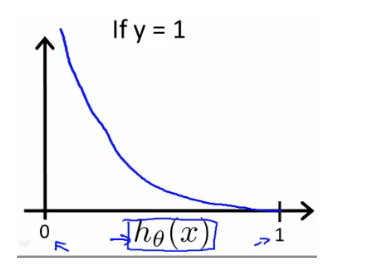
\includegraphics{logistic_cost_1}
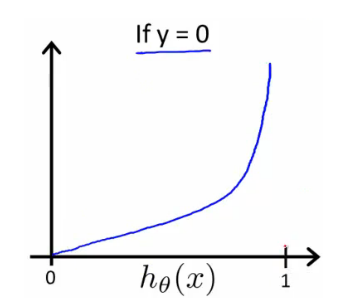
\includegraphics{logistic_cost_2}
\end{center}
\subsection{Descente de gradient}
Notre fonction de coût peut être synthétiser en une seule équation:
\begin{equation*}
cost(h_\theta(x),y) = -y log(h_\theta(x)) - (1-y) log(1-h_\theta(x))
\end{equation*}
Ainsi l'équation de la fonction de coût complète est :
\begin{equation*}
J(\theta) = -{1\over m} \sum_{i=1}^{m}
[y^{(i)}log(h_\theta(x^{(i)})+(1-y^{(i)})log(1-h_\theta(x^{(i)}))]
\end{equation*}
Donc une implémentation vectorisée est:
\begin{align*} & h = g(X\theta)\\ & J(\theta) = \frac{1}{m} \cdot \left(-y^{T}\log(h)-(1-y)^{T}\log(1-h)\right) 
\end{align*}
La forme générale de la descente de gradient étant : 
\begin{align*}& Repeat \; \lbrace \\ & \; \theta_j := \theta_j - \alpha \dfrac{\partial}{\partial \theta_j}J(\theta) \\ & \rbrace
\end{align*}
On obtient en appliquant la formule précédente:
\begin{align*} & Repeat \; \lbrace \\ & \; \theta_j := \theta_j - \frac{\alpha}{m} \sum_{i=1}^m (h_\theta(x^{(i)}) - y^{(i)}) x_j^{(i)} \\ & \rbrace 
\end{align*}
Avec pour implémentation vectorisée:
\begin{equation*}
\theta := \theta - {\alpha \over m}X^T(g(X\theta) - \overrightarrow{y})
\end{equation*}
\subsection{Classification multi-classe : "One vs All"}
Un problème de classification est dit multi-classe lorsque la classification n'est plus binaire. Ainsi, la répartition ce fait en plus de 2 ensembles. \newline
Exemple: Système de tagging d'emails, maladie qui touche un patient (pas malade, rhume, grippe),... 
\paragraph{One vs All}
On entraîne notre classificateur de régression logistique $h_\theta^{(i)}(x)$ pour chaque classe $i$ pour prédire la probabilité que $y=i$ \newline
Pour chaque nouvelle entrée $x$, pour faire une prédictinon on prend la classe $i$ qui maximise: 
\begin{equation*}
\max_i h_\theta^{(i)}(x)
\end{equation*}
\begin{center}
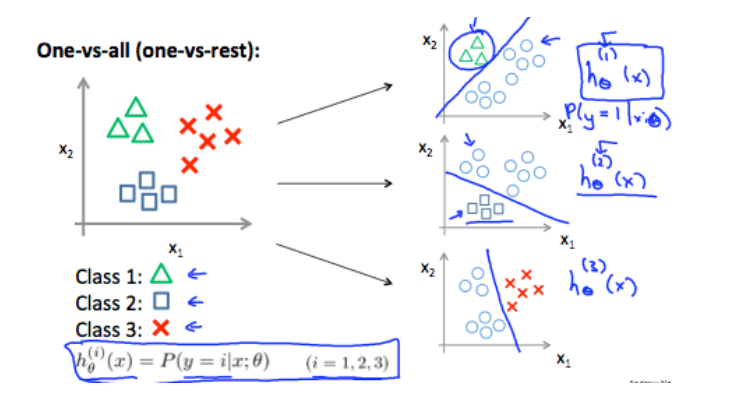
\includegraphics[scale=0.5]{onevsall}
\end{center}
\subsection{Optimisation avancée}
Il existe des algorithmes plus performants que la descente de gradient pour calculer et trouver le minimum d'une fonction de coût ("Conjugate gradient", "BFGS", and "L-BFGS"). \newline
Il y a des librairies qui implémentent ces algorithmes, il suffit simplement de leur fournir une fonction avec les formules pour chaque paramètres et pour la fonction de coût.\par
\newpage 
\section{Régularisation}
\subsection{Le problème du sur-apprentissage "Overfitting")}
Lorsque nous avons trop de paramètres, l'hypothèse peut bien s'adapter à notre ensemble de valeurs d'entraînement, mais généraliser de manière erronée de nouveaux exemples. \newline
Pour résoudre se problème on pourrait:
\begin{enumerate}

\item Reduire le nombre de paramètres (manuellement ou avec un algorithme de sélection)
\item Garder le même nombre de paramètres
\end{enumerate}
C'est ce que fait la \textbf{régularisation}, elle garde le même nombre de paramètres et réduit les valeurs de certains paramètres $\theta_j$ en les pénalisant \par
\subsection{Fonction de coût}
Pour déterminer quelles sont les paramètres que l'ont doit pénaliser, on modifie légèrement notre fonction de coût en ajoutant une nouvelle partie à notre équation ("regularization term") avec $\lambda$ qui représente le paramètre de régularisation, c'est à dire l'inflation du coût d'un des paramètres $\theta_j$. \par
Plus lambda est grand, plus la variable va coûter chère, donc pour résoudre notre équation de coût (i.e qui cherche à trouver la valeurs des paramètres $\theta_j$ qui la minimise) la valeur du paramètre $\theta_j$ va tendre vers 0. (i.e ne pas être pris en compte)
\begin{equation}
J(\theta) = {1\over 2m}[ \sum_{i=1}^{m} (h_\theta (x_i) - y_i)^2 + \lambda \sum_{j=1}^{n} \theta_j^{2}]
\end{equation}
\subsection{Régression linéaire régularisé}
On ne veut pas pénalisé le terme $\theta_0$, les équations pour la descente de gradient deviennent:
\begin{equation}
\theta_0 := \theta_0 - \alpha {1\over m} \sum_{i=1}^{m}(h_\theta(x^{(i)})-y^{(i)})x_0^{(i)}
\end{equation}
\begin{equation}
\theta_j := \theta_j - \alpha {1\over m} \sum_{i=1}^{m}(h_\theta(x^{(i)})-y^{(i)})x_j^{(i)} + {\lambda\over m} \theta_j
\end{equation}
Cette équation est aussi égale à celle si dessous après factorisation:
\begin{equation}
\theta_j := \theta_j(1-\alpha {\lambda\over m}) - \alpha {1\over m} \sum_{i=1}^{m}(h_\theta(x^{(i)})-y^{(i)})x_j^{(i)}
\end{equation}
On observe que le terme $(1-\alpha {\lambda\over m}) < 1$ lorsque $\lambda,m,alpha >0$.
On remarque donc que l'on a bien la même équation que précédemment et que le paramètre $\theta_j$ est diminué.\par
En ce qui concerne l'équation normale, la formule est la suivante:
\begin{equation}
\theta = X^{T}X+\lambda L^{-1}X^{T}y
\end{equation}
avec $L$, la matrice identité dont le premier terme de sa diagonale est nul.
\begin{equation}
X=
\begin{pmatrix}
x^{(1)^{T}} \\
... \\
x^{(m)^{T}} \\
\end{pmatrix}
\end{equation}
\begin{equation}
y=
\begin{pmatrix}
y^{(1)} \\
... \\
y^{(m)} \\
\end{pmatrix}
\end{equation}

Il est a noté que si $\lambda > 0$, alors la régularisation corrige le problème de non-inversibilité, puisque l'ajout de $\lambda L$ permet d'obtenir une matrice qui possède cette propriété.\par
\subsection{Régression logistique régularisé}
L'équation de coût pour la régression logistique devient:
\begin{equation*}
J(\theta) = -{1\over m} \sum_{i=1}^{m}
[y^{(i)}log(h_\theta(x^{(i)})+(1-y^{(i)})log(1-h_\theta(x^{(i)}))]+ {\lambda \over 2m} \sum_{j=1}^{n} \theta_j^{2}
\end{equation*}
Les équations de descente de gradient sont les mêmes que précédemment avec $h_\theta(x)= \frac{1}{1+e^{-\theta^{T}x}}$ 
\begin{equation*}
\theta_0 := \theta_0 - \alpha {1\over m} \sum_{i=1}^{m}(h_\theta(x^{(i)})-y^{(i)})x_0^{(i)}
\end{equation*}
\begin{equation*}
\theta_j := \theta_j(1-\alpha {\lambda\over m}) - \alpha {1\over m} \sum_{i=1}^{m}(h_\theta(x^{(i)})-y^{(i)})x_j^{(i)}
\end{equation*}
\newpage
\section{Réseaux de Neurones: Représentation}
Les réseaux de neurones ont été créés dans le but de simuler le fonctionnement des neurones au sein du cerveau. \par
 Un neurone possède deux fils de connexion, un d'entrée (les dendrites), et un de sortie (l'axone) pour communiquer avec les autres neurones. Ce n'est rien d'autre qu'une unité logistique. \par
Notations:
\begin{enumerate}
\item $a_i^{(j)}$ : "activation" de l'unité $i$ de la couche $j$
\item $\phi^{(j)}$ : Matrice de poids contrôlant le mappage de fonction de la couche $j$ à la couche $j+1$
\end{enumerate}
 \textbf{Propriété:} Si le réseaux possède $s_j$ unités logistiques pour sa couche $j$, et $s_{j+1}$ unités logistiques pour sa couche $j+1$, alors $\phi^{(j)}$ sera de dimensions: $$s_{j+1} X (s_j + 1)$$
Nous allons encapsuler dans une nouvelle variable $z$ les paramètres à l'intérieur de notre fonction $g$. Pour la couche $j=2$ et le noeud $k$
$$z_k^{(2)} = \theta_{k,0}^{(1)}x_0+...+\theta_{k,n}^{(1)}x_n$$
\par Sachant que : 
\begin{align*}x = \begin{bmatrix}x_0 \newline x_1 \newline\cdots \newline x_n\end{bmatrix} &z^{(j)} = \begin{bmatrix}z_1^{(j)} \newline z_2^{(j)} \newline\cdots \newline z_n^{(j)}\end{bmatrix}
\end{align*}
En remplaçant $x=a^{(1)}$, on obtient:
$$z^{(j)} = \theta^{(j-1)}a^{(j-1)}$$
Ainsi:
$$a^{(j)}=g(z^{(j)})$$
Finalement:
$$h_\theta(x) = a^{(j+1)} = g(z^{(j+1)})$$
L'intuition à avoir est de visualiser la fonction g(z) comme une sigmoïde (fonction de répartition de la loi logistique) et de dresser une table de vérité en fonction des entrées pour savoir quelle opération notre réseau de neurones construit.
\par Si l'on a besoin d'effectuer des opérations "complexes", il suffit d'associer les sous-opérations (AND, OR) en utilisant plusieurs couches ("hidden-layers")
\begin{center}
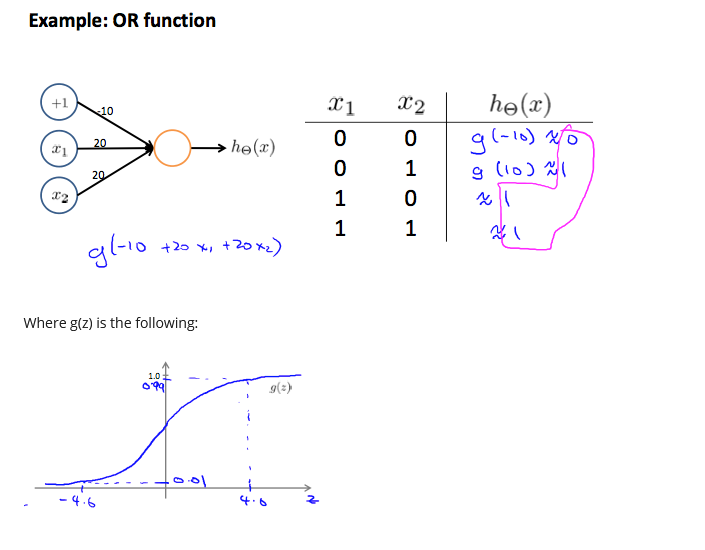
\includegraphics[scale=0.5]{neural_networks}

\end{center}
\newpage
\section{Réseaux de Neurones: Apprentissage}
\subsection{Fonction de coût}
Nous devons définir certaines variables:
\begin{itemize}
\item L = Nombre total de couches dans le réseau 
\item $s_l$ = Nombre d'unité logistique
\item K = Nombre d'unité en sortie (i.e, nombre de classe)
\item $h_\theta (x)_k$ = Hypothèse du résultats de la $k^{th}$ sortie
\end{itemize}
La fonction de coût, pour un réseau de neurones, est la suivante:
\begin{equation*} J(\Theta) = - \frac{1}{m} \sum_{i=1}^m \sum_{k=1}^K \left[y^{(i)}_k \log ((h_\Theta (x^{(i)}))_k) + (1 - y^{(i)}_k)\log (1 - (h_\Theta(x^{(i)}))_k)\right] + \frac{\lambda}{2m}\sum_{l=1}^{L-1} \sum_{i=1}^{s_l} \sum_{j=1}^{s_{l+1}} ( \Theta_{j,i}^{(l)})^2
\end{equation*}
\subsection{Algorithme de Rétro-propagation}
Le terme "rétro-propagation" est une terminologie des réseaux de neurones pour minimiser notre fonction de coût.
$$ min_\Theta J(\Theta)$$
C'est à dire qu'on cherche à minimiser $J$ en utilisant un ensemble du paramètre $\Theta$ qui est optimal.
Pour ce faire il nous faut calculer les dérivés partielles de $J(\Theta)$.
$$\frac{\partial J(\Theta)}{\partial \Theta_{i,j}^{(l)}}$$
\paragraph{Intuition}
Calculer $\delta_j^{(l)}$, l'erreur pour le nœud $j$ de la couche $l$
\paragraph{Algorithme}
Soit les variables suivantes
\begin{itemize}
\item Un jeu de données $\{(x^{1},y^{1}),...,(x^{m},y^{m})\}$
\item $\Delta_{ij}^{(l)} = 0 $ $\forall i,j,l$
\end{itemize}
\par Pour chaque jeu de données $(i=1:m)$, effectuer les étapes suivantes:
\begin{enumerate}
\item Établir $a^{(1)} = x^{(i)}$
\item Effectuer la propagation (cf. forward propagation) pour calculer $a^{(L)}$
\item En utilisant $y^{(i)}$, calculer $\delta^{(L)} = a^{(L)} - y^{(i)}$
\item Calculer $\delta^{(L-1)}$,...,$\delta^{(2)}$
\item Calculer $\Delta_{ij}^{(l)} := \Delta_{ij}^{(l)} + a_j{(l)}\delta_i^{(l+1)}$
\end{enumerate}
\par Finalement, calculer:
\begin{center}
$D_{ij}^{(l)} := \frac{1}{m} \Delta_{ij}^{(l)} + \lambda \Theta_{ij}^{(l)}$ si $j \neq 0$
\end{center}
\begin{center}
$D_{ij}^{(l)} := \frac{1}{m} \Delta_{ij}^{(l)}$ si $j = 0$
\end{center}
\par Sachant que:
$$\frac{\partial J(\Theta)}{\partial \Theta_{i,j}^{(l)}} = D_{ij}^{(l)}$$
\subsection{La Rétro-propagation en Pratique}
\paragraph{Dérouler les paramètres}
Si l'on souhaite obtenir toutes nos matrices dans un long vecteur, nous devons "dérouler" les matrices de la manière suivante (en MATLAB) pour les données à une fonction de minimisation de fonction de coût:
$$thetaVector = thetaVector = [ Theta1(:); Theta2(:); Theta3(:); ]$$
Pour retrouver les vecteurs d'origines si les dimensions sont les suivantes
\begin{itemize}
\item Theta1 (10x11)
\item Theta2 (10x11)
\item Theta3 (1x11)
\end{itemize}
$$Theta1 = reshape(thetaVector(1:110),10,11)$$
$$Theta2 = reshape(thetaVector(111:220),10,11)$$
$$Theta3 = reshape(thetaVector(221:231),1,11)$$
\paragraph{Vérifier le gradient}
Nous pouvons vérifier les valeurs de nos dérivées partielles pour la fonction de coût de la façon suivante:
$$\frac{\partial J(\Theta)}{\partial \Theta} =  \frac{J(\Theta + \epsilon) - J(\Theta - \epsilon)}{2\epsilon}$$

\paragraph{Initialisation aléatoire}
Nous devons initialiser les valeurs de $\Theta_{ij}^{(l)}$ dans l'intervalle $[-\epsilon, \epsilon]$ \par
En MATLAB, si Theta1 est une matrice de dimensions (10x11), on peut écrire le code suivant:
$$Theta1 = rand(10,11) * (2 * EPSILON) - EPSILON$$
\paragraph{En résumé}
D'abord il faut choisir une architecture pour notre réseau de neurones:
\begin{itemize}
\item Nombre d'unités en entrée = dimensions des features $x^{(i)}$
\item Nombre d'unités en sortie = nombre de classes
\item Nombre d'unités par couche intermédiaire (i.e, "hidden layer") = usuellement, le plus le mieux
\end{itemize}
Pour entraîner le réseau de neurones:
\begin{enumerate}
\item Initialiser les poids de manière aléatoire
\item Implémenter la propagation pour obtenir $h_\theta(x^{(i)}$
\item Implémenter la fonction de coût
\item Implémenter la rétro-propagation pour calculer les dérivés partielles
\item Utiliser la vérification de gradient pour confirmer que la rétro-propagation est correcte. Ne pas oublier de "désactiver" cette vérification par la suite
\item Utiliser la descente de gradient (ou une autre fonction ex: fminc) pour minimiser la fonction de coût
\end{enumerate}
\newpage
\section{Conseils pour appliquer les algorithmes de Machine Learning}
Pour débugger un algorithme d'apprentissage, dans le cas où l'on obtient des erreurs trop élevés sur les prédictions, on peut essayer les démarches suivantes:
\begin{itemize}
\item Avoir un plus grand jeu d'exemples
\item Essayer avec moins de features
\item Essayer d'ajouter des features
\item Essayer d'ajouter des features polynomiales
\item Essayer de diminuer/augmenter $\lambda$
\item \textbf{Diagnostiquer l'algorithme d'apprentissage}t
\end{itemize}
\subsection{Évaluer une hypothèse}
Pour vérifier si notre hypothèse sur-apprend le jeu de données (cf. "overfitting problem"), on peut séparer le jeu d'apprentissage en 2 parties: \newline 
Un jeu d'exemples (70\% de l'ensemble) et un jeu test (30\%).
\par Avec ces deux ensembles, la procédure pour évaluer une hypothèse est la suivante:
\begin{enumerate}
\item Apprendre $\Theta$ et minimiser $J_{train}(\Theta)$ en utilisant le jeu d'exemple classique
\item Calculer l'erreur de test sur le jeu de test $J_{test}(\Theta)$ 
\end{enumerate}
\subsubsection{Regression linéaire}
Dans le cas de la régression linéaire, l'erreur test, sur le jeu de test est :
$$J_{test}(\Theta) = \frac{1}{2m_{test}} \sum_{i=1}^{m_{test}} (h_{\Theta}(x_{test}^{(i)}) - y_{test}^{(i)})^2$$
\subsubsection{Regression logistique (classification)}
Dans le cas de la régression logistique, l'erreur test, sur le jeu de test est :
\newline 
$err(h_\Theta(x),y) = 1$ if $h_\Theta(x) \geq 0.5$ and $y=0$
\newline
$err(h_\Theta(x),y) = 1$ if $h_\Theta(x) < 0.5$ and $y=1$
\newline
$err(h_\Theta(x),y) = 0$ otherwise
\par La moyenne des erreurs de test pour le jeu de test est :
$$TestError = \frac{1}{m_{test}}  \sum_{i=1}^{m_{test}} err(h_{\Theta}(x_{test}^{(i)}) - y_{test}^{(i)}) $$
\subsubsection{Sélectionner le modèle}
Pour choisir le modèle de notre hypothèse, on peut tester chaque degré de polynôme et regarder l'erreur du résultat. Une manière de faire est de diviser le jeu d'entraînement en trois parties:
\begin{itemize}
\item Un jeu d'entraînement classique (60\%)
\item Un jeu de validation (20\%)
\item Un jeu de test (20\%)
\end{itemize}
On peut maintenant avoir trois valeurs d'erreurs pour chaque sous-jeu en suivant la méthode suivante:
\begin{enumerate}
\item Optimiser le paramètre $\Theta$ en utilisant le jeu d'entraînement classique pour chaque degré de polynôme
\item Trouver le degré de polynôme qui possède la plus petite valeur d'erreur sur le jeu de validation
\item Estimer la généralisation de l'erreur sur le jeu de test
\end{enumerate}
De cette manière le degré du polynôme $d$ (i.e, une variable) n'a pas été entraîné sur le jeu de test.\par
\subsection{Biais vs Variance}
Un problème de sous-apprentissage est du à un biais élevé. Et un problème de sur-apprentissage est du à une variance élevée. \par
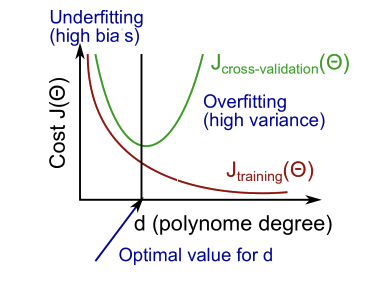
\includegraphics{biasvsvariance}
\subsection{Courbe d'apprentissage}
Afficher les courbes d'apprentissage permet de se rendre compte de la présence d'un haut biais ou bien d'une variance élevée.
\subsubsection{Fort biais}
Si un algorithme d'apprentissage souffre d'un fort biais, avoir un plus grand jeu de données n'aiderait pas (à lui seul) à régler le problème. \par
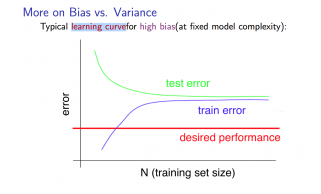
\includegraphics{highbias}
\subsubsection{Forte variance}
Si un algorithme d'apprentissage souffre d'une variance élevée, avoir un plus grand jeu de données aidera (à lui seul) à régler le problème. \par
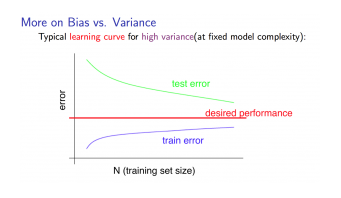
\includegraphics{highvariance}
\subsection{Focus sur les conseils}
Si l'on revient sur les démarches précédemment établies, nous pouvons faire les conclusions suivantes:
\begin{itemize}
\item Avoir un plus grand jeu d'exemples \textbf{corrige la variance élevée}
\item Essayer avec moins de features \textbf{corrige la variance élevée}
\item Essayer d'ajouter des features \textbf{corrige un biais élevé}
\item Essayer d'ajouter des features polynomiales  \textbf{corrige un biais élevé}
\item Essayer de diminuer $\lambda$ \textbf{corrige un biais élevé}
\item Essayer d'augmenter $\lambda$ \textbf{corrige la variance élevée}
\end{itemize}
\paragraph{Réseaux de neurones et sur-apprentissage}
Un "petit" réseau de neurones sera enclin à sous-apprendre. Tandis qu'un "grand" réseau de neurones sera enclin à sur-apprendre. (utiliser la régularisation $\lambda$ pour corriger ce problème.
\newpage
\section{"Support Vector Machine" (Machine à vecteurs de support)}
Les machines à vecteurs de support sont un ensemble de techniques d'apprentissage supervisé destinées à résoudre des problèmes de discrimination et de régression.\par
La fonction de coût est légèrement différente:
\begin{center}
$$\min_\theta C\sum_{i=1}^{m}[y^{(i)}cost_1(\theta^{T}x^{(i)})+(1-y^{(i)})cost_0(\theta^Tx^{(i)})]+ \frac{1}{2}\sum_{i=1}^{n}\theta_j^2$$
\end{center}
Avec $C=\frac{1}{\lambda}$, $cost_1(x)$ et $cost_0(x)$:
\begin{center}
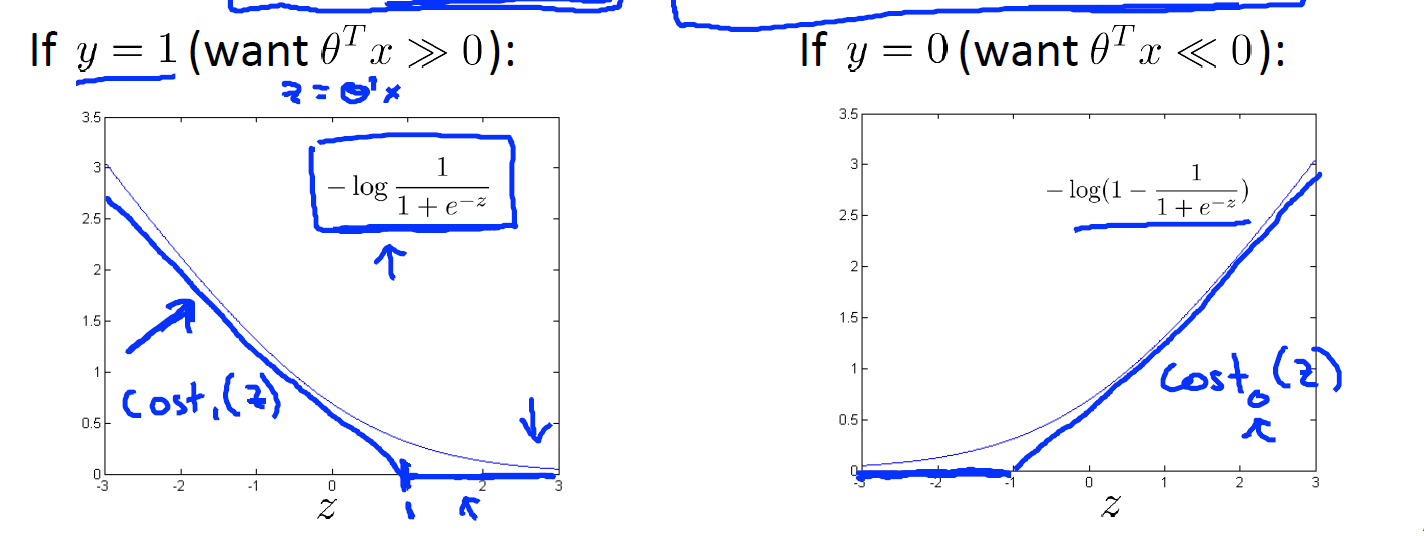
\includegraphics[scale=0.3]{svm}
\end{center}
La particularité des SVM est d'être des séparateurs à vaste marge. ("Large Margin Classifier")\par
\subsection{Kernel}
L'astuce du noyau ("Kernel trick") permet d'adapter les SVM pour développer des classificateurs non-linéaire complexe.\par
Le principe est de définir si un point est proche d'un point de repère, si c'est le cas, lui attribuer la valeur 1, sinon, lui attribuer la valeur 0.\par
Exemple:
$$ f_1=similarity(x,l^{(1)})=exp(-\frac{norme(x-l^{(1)})}{2\sigma^2}) = exp(-\frac{\sum_{j=1}^{n}(x_j-l_j^{(1)})^2}{2\sigma^2})$$
La fonction de similarité est en réalité le "Gaussian Kernel".
Pour choisir les points de repère, on prendra les $x^{(i)}$ du jeu d'exemple, et on remplacera les $x$ par des $f$ avec:
$$f_i=similarity(x,l^{(i)})$$
\subsection{Influence des paramètres}
\paragraph{C} Une grande valeur de C implique, un faible biais et une grande variance. Une petite valeur de C au contraire, implique un fort biais et une faible variance.
\paragraph{$\sigma^2$} Une grande valeur de $\sigma^2$ (pour laquelle les features $f_i$ varient de manière fluide) implique un fort biais et une faible variance. Une faible valeur de $\sigma^2$ implique un faible biais et une grande variance.\par
\subsection{Régression logistique vs SVM}
Soit les variables suivantes:
\begin{itemize}
\item n = le nombre de features
\item m = le nombre d'exemples d'entraînement
\end{itemize}
Si $n>>m$ alors il faut utiliser la regréssion logistique, ou SVM sans kernel. ("linear kernel").\newline
Si $n$ est petit et $m$ est moyen, alors il faut utiliser SVM avec le "Gaussian kernel". \newline
Si $n$ est petit et $m$ est grand, alors il faur ajouter des features pour ensuite utiliser la régression logistique ou SVM sans kernel. \par
\newpage
\section{Apprentissage Non-Supervisé}
Dans un problème d'apprentissage non-supervisé, le jeu d'exemples n'a pas de label, on ne sait pas à quelles classes les données appartiennent. Cependant on peut encore distinguer des clusters et observer une tendance pour notre nuage de point. \par
L'algorithme de partitionnement des données (i,e clustering) est un exemple d'algorithme d'apprentissage non-supervisé.\par
\subsection{Algorithme de partionnement des données: K-Means}
K-Means est un algorithme itératif qui fait deux choses:
\begin{enumerate}
\item D'abord il effectue une étape d'assignation de cluster
\item Ensuite il bouge les centres des clusters. Il fait la moyenne des centres des points appartenant au cluster et bouge le centre du cluster
\end{enumerate}
Ensuite il itère sur ces deux opérations, jusqu'à convergence.
Au départ les centre des clusters sont générés aléatoirement.\par
Notation :
\begin{itemize}
\item $c^{(i)}$ = index du cluster auquel l'exemple $x^{(i)}$ est assigné
\item $\mu_k$ = centre du cluster $k$
\item $\mu_c^{(i)}$ = centre du cluster auquel l'exemple $x^{(i)}$ a été assigné
\end{itemize}
\paragraph{Objectif d'optimisation} L'algorithme K-Means tente de minimiser la fonction de coût suivante:
$$J(c^{(1)},...c^{(m)},\mu_1,...,\mu_K) = \frac{1}{m}\sum_{i=1}^{m}Norme_2(x^{(i)}-\mu_c(i))$$
C'est ce que fait l'algorithme, dans un 1er temps en minimisant les variables $c^{(i)}$ et dans un 2nd temps en minimisant les variable $\mu_i$
\paragraph{Initialisation aléatoire} Nous devons avoir $K < m$ (moins de cluster que d'exemple dans le jeu d'exemples). On prend aléatoirement K exemple du jeu d'exemples et les centres de ses clusters seront égaux aux centres des valeurs du jeu d'exemples choisi. Si on ne veut pas être coincer dans des optimums locaux, il faut appliquer cette méthode de multiple fois.
\paragraph{Choisir le nombre de clusters} On peut essayer la "Elbow Method", qui consiste à choisir K si pour une certaine valeur, les valeurs suivantes font décroître la fonction de coût que très légèrement. Sinon, il faut réfléchir à ce que l'on souhaite représenter et faire un choix.\par
\subsection{Réduction Dimensionnelle}
Permet de comprimer les données (optimiser les temps de calculs) et d'améliorer la visualisation des données. (moins de dimensions, donc plus compréhensible) \par
\subsection{Analyse en composantes principales (PCA)}
Algorithme le plus utilisé pour réduire la dimension d'un jeu de données.\par
Pour réduire un problème n-dimensionnelle à un problème k-dimensionnelle il faut: trouver $k$ vecteurs $u^{(1)},...,u^{(k)}$ sur lesquels projeter les données, pour minimiser l'erreur de projection. (plus courte distance entre le vecteur et le points, différent de la régression linéaire)
\paragraph{Algorithme} Pour réduire des données n-dimensionnelle à des donnes k-dimensionnelle, il faut calculer la matrice de covariance:
$$\Sigma = \frac{1}{m} \sum_{i=1}^{n}(x^{(i)})(x^{(i)})^T$$
Il faut ensuite calculer les vecteurs propres de la matrice $\Sigma$ :
$$[U,S,V] = svd(\Sigma)$$
De la matrice $U$, on ne récupère que les $k$ premiers vecteurs colonnes, appelons-la $U_{reduce}$, on peut obtenir un vecteur $z$ tel que:
$$z=U_{reduce}^Tx$$
Ne pas oublier d'effectuer au préalable la moyenne normalisé et le feature scaling (optionnel)
\paragraph{Reconstruire le modèle} Pour revenir au modèle de base à partir du modèle compressé, il suffit de faire la transformation suivante:
$$X= U_{reduce}Z$$
\paragraph{Choisir le nombre de composantes principales} Pour choisir le nombre de composantes principales (i.e, la valeur de la variable $K$) au veut que 99\% de la variance soit retenue:
$$\frac{Average_squared_projection_error}{Total_variation_in_the_data} = \frac{\frac{1}{m}\sum_{i=1}^{m}Norme_2(x^{(i)}-x_{approx}^{(i)})}{\frac{1}{m}\sum_{i=1}^{m}Norme_2(x^{(i)})} \leq 0.01$$
Ce qui revient à faire:
$$
\frac
{\sum_{i=1}^{k}S_{ii}}
{\sum_{i=1}^{m}S_{ii}}
\geq
0.99
$$
\newpage
\section{Détection d'anomalies}
Un algorithme de détection d'anomalies qui fonctionne avec la loi normale est le suivant:
\begin{enumerate}
\item Choisir une feature $x_i$ que vous pensez être anormal
\item Mettre en forme les paramètres 
$$\mu_j = \frac{1}{m} \sum_{i=1}^{m}x_j^{(i)}$$
$$\sigma^2 = \frac{1}{m} \sum_{i=1}^{m}(x_j^{(i)}-\mu_j)^2$$
\item Pour un nouvel exemple, calculer $p(x)$:
$$p(x)=\prod_{j=1}^{n}p(x_j;\mu_j;\sigma^2) = \prod_{j=1}^{n} \frac{1}{\sqrt{2\pi\mu_j}}exp(-\frac{(x_j-\mu_j)^2}{2\sigma_j^2})$$
Détecter comme anomalie si $p(x) < \epsilon$
\end{enumerate}
\paragraph{Détection d'anomalies vs Apprentissage supervisé} On utilise  l'algorithme de détection d'anomalies quand le jeu d'exemple contient un très petit nombre d'exemple positif ($y = 1$) et un grand nombre d'exemples négatifs ($y=0$). Dans le cas contraire, on utilise un algorithme d'apprentissage supervisé.
\newpage
\section{Systèmes de Recommandations}
Les systèmes de recommandations permettent de définir si un utilisateur va potentiellement aimer un contenu, en fonction de ses intérêts communiqué via de précédentes évaluations. \par
\paragraph{Formulation d'un problème: Recommandation de films} On définit les variables suivantes
\begin{itemize}
\item $r(i,j) = 1$ si l'utilisateur $j$ a évalué le film $i$
\item $y^{(i,j)}$ = évaluation (0 à 5 étoiles) de l'utilisateur $j$ pour le film $i$. (Sinon $y=undefined$)
\item $\theta^{(j)}$ vecteur de paramètres pour l'utilisateur $j$
\item $x^{(j)}$ = vecteur de features pour le film $i$
\item Pour l'utilisateur $j$, le film $i$, la prédiction d'évaluation est:
$$(\theta^{(j)})^T(x^{(j)})$$
\item $m^{(j)}$ = nombre de films évalué par l'utilisateur $j$
\end{itemize}
Pour apprendre $\theta^{(j)}$ (pour un utilisateur):
$$\min_{\theta^{(j)}} \frac{1}{2}\sum_{i:r(i,j)=1}((\theta^{(j)})^T(X^{(i)})-y^{(i,j)})^2 + \frac{\lambda}{2} \sum_{k=1}^{n} (\theta_k^{(j)})^2$$
\newpage
\section{Descente de gradient avec des grands jeux de données}
L'algorithme de descente de gradient est un algorithme coûteux (forte complexité temporelle). Pour chaque itération on parcours tous les exemples du jeu de données. Ainsi, il existe des variantes à cet algorithme de descente de gradient:
\begin{enumerate}
\item "stochastic gradient descent"
\begin{center}
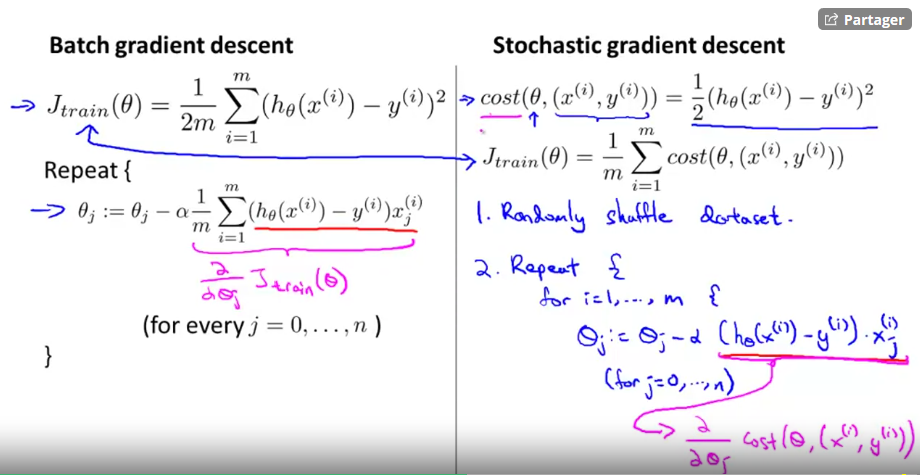
\includegraphics[scale=0.4]{stochastic}
\end{center}
\item "mini-batch gradient descent"
\begin{center}
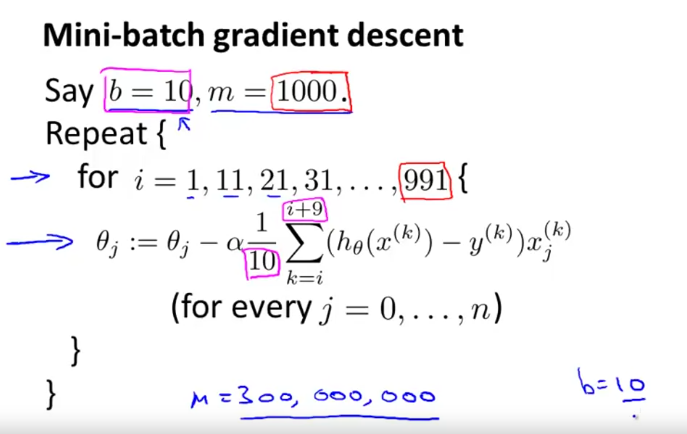
\includegraphics[scale=0.5]{minibatch} 
\end{center}
\end{enumerate}
\paragraph{Map-Reduce} C'est un patrons de conception qui permet de diviser le jeu de données en plusieurs parties, pour traiter les données sur différents ordinateurs (ou cœur logique) et de les regrouper par la suite, dans le but de traiter les données plus rapidement. \par
\newpage
\section{Application: Reconnaissance d'images}
Pour extraire des informations d'une image (personne, texte, ...), il faut exécuter la pipeline suivante dans le cas d'un algorithme de reconnaissance de textes:
\begin{enumerate}
\item Détecter les zones de texte
\item Segmenter les chaînes de caractères
\item Reconnaître chaque caractère
\end{enumerate}
Pour arriver à détecter les zones de texte, il faut utiliser la méthode dite de la fenêtre glissante. C'est à dire qu'il faut essayer avec plusieurs tailles de rectangle différentes, d'identifier des objets en avançant chaque rectangle d'un pas (ex: 1px, 4px, 8px). A la fin de ce processus, on obtient les différentes localisation des zones qui comportent nos objets.\par
Pour arriver à segmenter des chaînes de caractères. On applique le même processus. Sachant qu'un exemple est positif (i.e, $y=1$) lorsque la fenêtre contient une séparation entre deux caractères (un espace vide).\par
Enfin pour arriver à reconnaître un caractère, il suffit d'appliquer un algorithme d'apprentissage supervisé étudié précédemment.
\end{document}

